% kapitel4.tex

\chapter{Preselection in the Boosted Channel}

\section{Event Preselection}
\label{Event Preselection}
For the Monte-Carlo samples used in this analysis a specific preselection is chosen.\\
In table \ref{Event preselection} the different requirements are listed, which are part of this preselection. 

\vspace{0.5cm}

\begin{table}
\centering
\setlength{\tabcolsep}{3cm}
\begin{tabular}{|c|} 
\hline
\textbf{Event preselection} \\
\hline
\hline
\vspace{-0.3cm}
\\
Z boson candidate preselection:\\
\vspace{-0.1cm}
\footnotesize{$\bullet$ pair of opposite sign leptons (same flavor)} \\

\footnotesize{$\bullet$ $\mid m_{l^{+} l^{-}} - m_{Z} \mid$ < \SI{10}{GeV}} \\
\\
\vspace{-0.9cm}
\\
\hline
\vspace{-0.3cm}
\\
$\geq 2$ jets \\
\vspace{-0.4cm}
\\
$\geq$ 2 b-tags\\
\vspace{-0.4cm}
\\
= 2 leptons \\
\hline
\end{tabular}
\caption{Preselection criteria.}
\label{Event preselection}
\end{table}


The first aspect is the Z boson candidate preselection. 
According to the studied leptonic decay channel of the Z boson this includes a reconstructed Z candidate mass with \SI{10}{GeV} around the Z pole resulting from two opposite sign leptons with same flavor.
In this analysis only electrons and muons are considered in the Z candidate reconstruction and not the $\tau$ lepton or neutrinos.
Figure \ref{Zmass} shows the distribution of the reconstructed Z mass. 
Both signal and background are presented in one plot and are normalized to unity. 
The background is illustrated as colour filled histogram with a specific colour for each background process, which is listed in the legend.
The different background processes are stacked, which means that the histograms of the different background processes are added . 
The signal is shown as solid red and blue line for the BBS and TTS process.
In the legend the weighted number of events is displayed in brackets next to each process.
Furthermore the statistical uncertaintys are shown as vertical lines.
The shape of the distribution looks as expected because it displays a pole mass distribution which is smeared because of detector resolution.
Processes including a real Z boson, like the signal and Z+jets processes, have a peak at the Z mass. 
The \ttbar{} background process has no peak at the Z pole mass which is as anticipated as well because the leptons result from independent W boson decays.\\

\begin{figure}
\centering
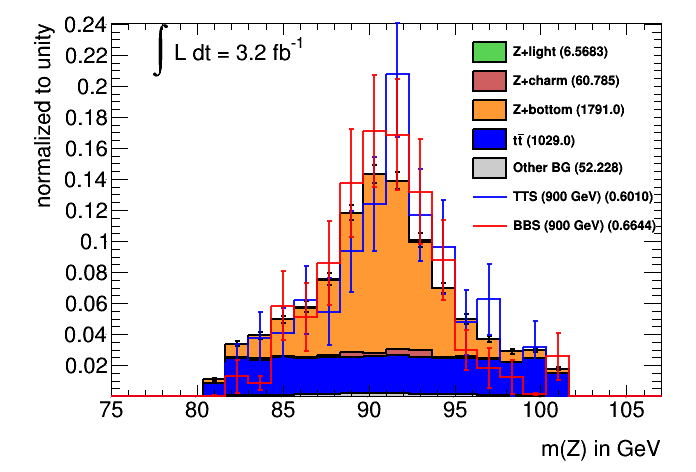
\includegraphics[width=8cm]{figures/Zmass.png}
\caption{Distribution of the reconstructed Z boson mass after the preselection. 
Both signal and background are presented and the distributions are normalized to unity.
The weighted number of events is displayed in the legend in brackets next to the processes. 
The number of events are expected for a integrated luminosity $\int{Ldt}$ = \SI{3,2}{fb^{-1}} }.
\label{Zmass}
\end{figure}

Furthermore, in the preselection at least two jets with $|\eta | < 2.5$ and $p_{T} < \SI{25}{GeV}$ are required.
The $p_{T}$ requirement should ensure that the jets are calibrated and the $\eta$-region is limited because the detector resolution in this $\eta$-region is better than in regions with $|\eta | > 2.5$.  
Because of the specific decay topology, two or more b-tags for the jets are expected.
One b-jet results straight from the vector-like quark decays T\texorpdfstring{$\longrightarrow$}~Wb and B \texorpdfstring{$\longrightarrow$}~Zb.
The other is caused by the third generation top quark decays t\texorpdfstring{$\longrightarrow$}~Wb.
The top quarks are the decay products of the second vector-like quarks with T\texorpdfstring{$\longrightarrow$}~Zt and B\texorpdfstring{$\longrightarrow$}~Wt.\\  
The last aspect of the preselection listed in table \ref{Event preselection}  is the requirement of exact two leptons. 
This guarantee that the analysis is performed in the dilepton channel. There are analysis in the trilepton channel, too.



\section{Boosted Analysis Strategy}
The samples are simulated with a vector-like quark mass of $m_{T/B} =$ \SI{900}{GeV}. 
Because of the massive vector-like T and B the decay products have high transverse momenta. 
Caused by the high transverse momenta the particles of the subsequent decays are strongly collimated. 
This situation is illustrated in figure \ref{boosted} for a top quark decay.
The figure shows the decay for a low and a high top-quark $p_{T}$.
As mentioned before, the figure shows that the decay products of the top-quark are collimated for a high top-quark $p_{T}$.\\

\begin{figure}
\centering
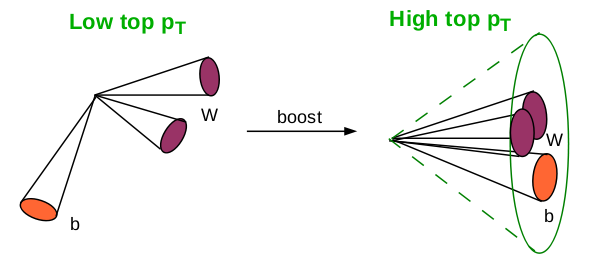
\includegraphics[width=9cm]{figures/boost.png}
\caption{Representative figure for a top quark decay with a high and a low top $p_{T}$ \cite{boosted}.}
\label{boosted}
\end{figure}

This collimated structure of the particles have an inpact on the jet clustering algorithms used in the ATLAS experiment.
Jets can for example be clustered with the anti-$k_{t}$ jet clustering algorithm \cite{antikt}.  
The anti-$k_{t}$ algorithm clusters soft particles around a hard particle within a given radius and forms conical jets. 
If two hard particles are located within an area closer than R, the clustering algorithm is not able to form a smooth circular shape around the hard particles.  
For a low top-quark $p_{T}$, a $R = 0.4$ can be used.
In the high $p_{T}$ regions, it is probable, that the jets from the top decay, which are clustered with $R = 0.4$,  merge because the one decay product can be close to another decay product. 
Hence as mentioned before the anti-$k_{t}$ algorithm is not able to form smooth circular shapes. 
To avoid this problem the boosted analysis strategy can be used for high top-quark transverse momenta.
The idea of the boosted analysis strategy is to cluster one jet which has all decay products of a boosted particle in it.
The area, where the decay products of a particle are located can be estimated with the formula $R \approx \frac{2m}{p_{T}}$, with m and $p_{T}$ for the mass and transverse momentum of the motherparticle and R the distance of the childparticle.
In the boosted analysis a radius of $R = 1.0$ for the cluster algorithm is used. 
A combined result from the top quark mass measurement is $m_{t} =$ \SI{173.34 \pm 0.76}{GeV} \cite{topmass}.
Using the formula mentioned before the boosted analysis is sensibel for a $p_{T}$ of the top quark about \SI{350}{GeV} and more. 
The boosted analysis strategy can be used for a decay of a boosted W boson, too.\\
In this analysis jets clustered with  $R = 1.0$ are used.   
These jets are called large-R jets. 
Large-R jets offer the possibility to introduce top- and boson tagging.
The top-tagger \cite{toptag} utilized in this analysis uses two variables for the top-jet identification, the invariant mass of the jet constituents $m_{jet}$ and the subjettiness ratio $\tau_{32}$, which discribes how adequate the jet can be interpretated as jet with three constuents.
For the analysis the 80\% signal efficiency working point for the top-tagger is choosen. 
The W-tagger \cite {Wtag} works with three substructure variables in combination with a groomed jet mass window.
The chosen working point of the W-tagger has 50\% signal efficiency. 
Table \ref{calibration} contains different conditions large-R jets have to fulfill to ensure that they are calibrated.

\begin{table}[h!]
\centering
\setlength{\tabcolsep}{3cm}
\begin{tabular}{|c|} 
\hline
\textbf{Large-R jet only calibrated for:}\\
\hline
\hline
$p_{T}$(large-R jet) $\geq \SI{200}{GeV}$\\
$\mid \eta \mid < 2.0$ \\
m(large-R jet) $> \SI{50}{GeV}$\\
\hline
\end{tabular}
\caption{Minimum criteria for large-R jets.}
\label{calibration}
\end{table}

Only calibrated large-R jets are considered.
Furthermore large-R jets within an area of $\Delta R < 1.0$ around the Z candidate reconstructed from two electrons are discarded in this analysis.
Figure \ref{deltaR} shows the distribution of the $\Delta R$ between all large-R jets in an event and the Z candidate of this event.

\begin{figure}
\centering
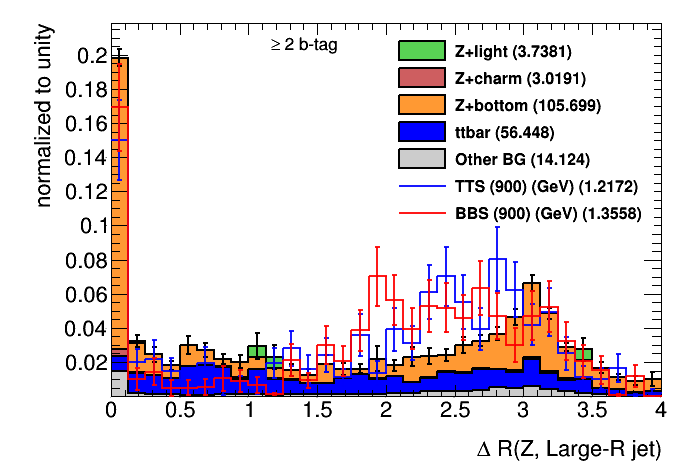
\includegraphics[width=8cm]{figures/deltaR.png}
\caption{Distribution of the $\Delta R$ of the large-R jets and the Z boson candidate after the preselection. 
Both signal and background are presented and the distributions are normalized to unity. 
The weighted number of events is displayed in the legend in brackets next to the processes. 
The number of events are expected for a integrated luminosity $\int L dt$ = \SI{3.2}{fb^{-1}}}.
\label{deltaR}
\end{figure}

The distribution has a clear peak at $\Delta R = 0$, which illustrates that the decay products of the Z candidate are often misidentified as large-R jets.
This is caused by the electrons which can be misidentified as large-R jets because of a simular signature in the detector.
Because of that, it is reasonable to ignore all large-R jets within an area of $\Delta R < 1.0$ around the Z candidate reconstructed from two electrons to avoid that they are treated as large-R jets in the analysis.
This requirement is called overlap removal.



      



\section{Basic Selection Implied by the Boosted WbZt Topology  }
\label{basic selection}
The decay topologys TT \texorpdfstring{$\longrightarrow$}~ZtWb and BB \texorpdfstring{$\longrightarrow$}~ZbWt for the optimization studies in this analysis are defined as mentioned before. 
Because of the specific products of the vector-like quark decays further selection can be added to the preselection discussed in section \ref{Event preselection}.       
It is reasonable that at least two large-R jets should be required considering that there is one top quark and one W boson, which could lead to large-R jets. 
Events without at least one top- and W-tag should also be rejected.  
Figure \ref{ljetmult} shows the multiplicity of the large-R jets.

\begin{figure}
\centering
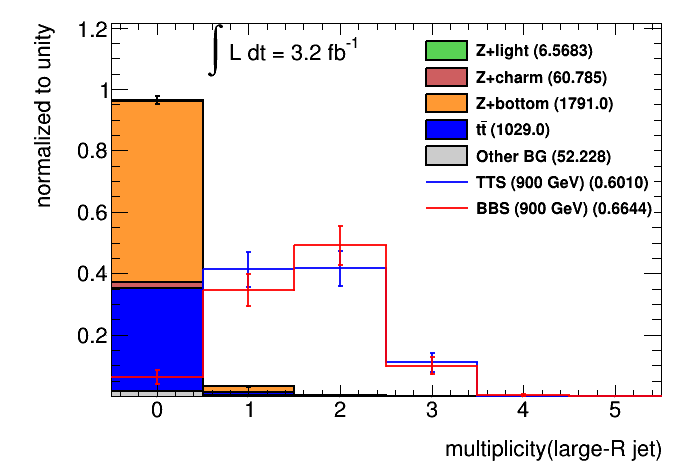
\includegraphics[width=8cm]{figures/multipliljet.png}
\caption{Plot for the large-R jet multiplicity after the preselection. 
Both signal and background are presented and the distributions are normalized to unity. 
The weighted number of events is displayed in the legend in brackets next to the processes. 
The number of events are expected for a integrated luminosity $\int L dt$ = \SI{3.2}{fb^{-1}}}
\label{ljetmult}
\end{figure}

As expected, the background processes mostly have no large-R jets because in most cases the $p_{T}$ of the particles is not high enough to produce large-R jets with the minimum requirements (see table \ref{calibration}).
The decay topology considered in this analysis gives reason to expect two large-R jets resulting from the boosted top-quark and W boson decays.
Therefore the signal distribution looks not like expected caused by the fact that about 40 \% of the events only have one large-R jets. 
An explanation for the distribution could be, that the W bosons from T \texorpdfstring{$\longrightarrow$}~Wb and B \texorpdfstring{$\longrightarrow$}~Wt  can be located in an area of $\Delta R = 1.0$ around the Z candidate and therefore are ignorated caused by the overlap removal mentioned earlier.
For the BBS signal process the case mentioned before is also possible for the jet resulting from the top quark.
Furthermore for the TTS signal process it is possible that the decay products of the W-boson and the top quark are clustered in one large-R jet because they are in an area of $\Delta R = 1.0$.\\
The requirement of two large-R jets selects the background from the signal and rejects a lot of background.
There are also a lot of signal events which are ignored as dicussed before.
A representation for the distribution of the top- and W-tag multiplicity can be found in  figure \ref{topmultipli} and \ref{bosonmultipli}.

\begin{figure}[h]
    \centering
    \resizebox{0.46\columnwidth}{!}{
    \begin{subfigure}{.49\textwidth}
      \centering
      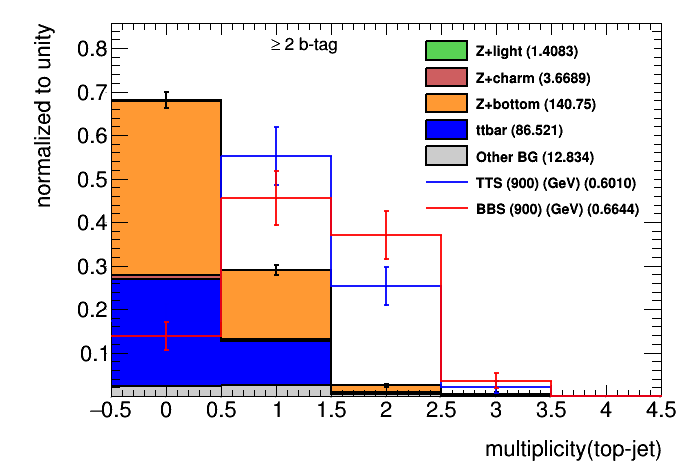
\includegraphics[width=.99\linewidth]{figures/topmultiplicity.png}
      \caption{}
      \label{topmultipli}
    \end{subfigure}
    }
    \resizebox{0.46\columnwidth}{!}{
    \begin{subfigure}{.49\textwidth}
      \centering
      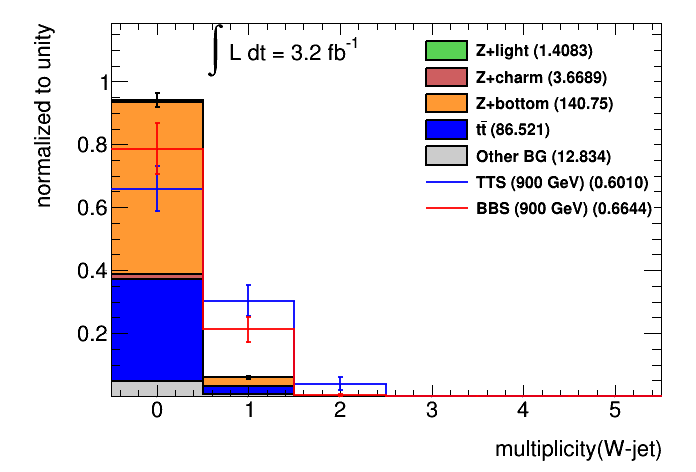
\includegraphics[width=.99\linewidth]{figures/Wmultiplicity.png}
      \caption{}
      \label{bosonmultipli}
    \end{subfigure}
    }
    \caption{Plot for the top-tagged large-R jet multiplicity (a) and W-tagged large-R jet multiplicity (b) . 
Both signal and background are presented and the distributions are normalized to unity. 
The weighted number of events is displayed in the legend in brackets next to the processes. 
The number of events are expected for a integrated luminosity $\int L dt$ = \SI{3.2}{fb^{-1}}.}
    \label{fig::stop}   
\end{figure}




The plot for the top-tag multiplicity shows that most background events do not have a top-tagged large-R jet.
That is reasonable if the Z+jets backgrounds are regarded because in these processes no top quark is included. 
The \ttbar{} process should also have no top-tag because the W bosons produced by the top quarks decay in the leptonic decay channel because there are two leptons required.
Therefore only  b-tagged jets are produced.
If the leptons resulting from the Z for the Z+jets backgrounds are not in an area $\Delta R = 1.0$ around the Z candidate they are not rejected by the overlap removal.
For the \ttbar{} process it is also possible that the leptons from the W boson decays are counted as large-R jets.
Hence there are some events with one top-tag in the background distribution.\\
The signal distribution looks not like assumed because there are a lot of events having two top-tagged large-R jets.
This is caused by the fact that the top-tagger also tag the large-R jet resulting from the W-boson as top-tag, because the lower limit for the $m_{inv}$ (mentioned in section 4.2) is at \SI{70}{GeV} for the used top-tagging working point.
The low limits for the top-tagger are chosen to avoid, that large-R jets resulting from a top, which only include the W boson, are ignored.
Figure \ref{topobosontag} shows the multiplicity fot the W-tagged jets which are not also top-tagged.

\begin{figure}[h!]
\centering
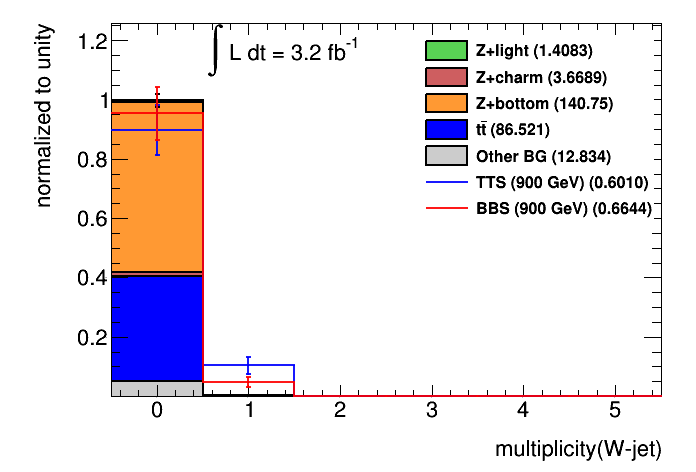
\includegraphics[width=8cm]{figures/Wotoptag.png}
\caption{Plot for the W-tag multiplicity with requiring a top-tag veto. The preselection is implemented. 
Both signal and background are presented and the distributions are normalized to unity. 
The weighted number of events is displayed in the legend in brackets next to the processes. 
The number of events are expected for a integrated luminosity $\int L dt$ = \SI{3.2}{fb^{-1}}}.
\label{topobosontag}
\end{figure}

The distribution confirms the argumentation mentioned before, because it shows that almost none W-tagged jets are not top-tagged at the same time.
The number of events without a top-tagged large-R jet can be explained with the signal efficiency of the used top-tagger.\\
The background distribution for the W-tagged large-R jets (figure \ref{bosonmultipli}) be explained with the same argumentation as for the top-tag multiplicity.
For the signal processes there is a high amount of events without W-tagged large-R jet (about 80 \% for TTS and 65 \% for BBS), which is not as expected.
This could be caused by the argumentation mentioned before that the large-R jet pruduced by the W-boson is ignored because of the overlap removal.
In addition to that the boson-tagger doesn't work perfectly but has an efficiency of 50 \%.\\
After demanding all three parts of the basic selection implied by the boosted WbZt topology, a lot of background is rejected, which becomes obvious in the three discributions described before.
The unweighted number of events, which means the real number of Monte-Carlo events, without any weights applied , and the weighted number of events (discussed in section \section{samples}) for signal and background after the basic selection is listed in table \ref{numberoevents}.
The listed numbers reveal that after the event preselection and basic selection there are for both signal and background very  low numbers of events.
An optimization study without enough statistic is not convincing because the distributions subject to large statistical uncertainties.
Therefore the optimization study in this analysis is performed without requiring at least one W-tag.
The number of events after the basic selection is much higher for both signal and background without this requirement.
These number of events both weighted and unweighted are listed in table \ref{numberoevents1}.

\begin{table}
\centering
%\setlength{\tab}{\textwidth}
\resizebox{0.8\columnwidth}{!}{
\begin{tabular}{|c|c|c|} 
\hline
\textbf{Process} & \textbf{Unweighted number of events} & \textbf{Weighted number of events}  \\
\hline
\hline
Z+light & 3 & 0.0005\\
Z+charm & 2 & 0.0060\\
Z+bottom & 77 & 0.1680\\
ttbar{} & 6 & 0.3739\\
Other BG & 1331 & 0.3298\\
TTS & 214 & 0.1094\\
BBS & 176 & 0.1089\\
\hline
\end{tabular}
}
\caption{Unweighted and weighted number of events for signal and background processes after requiring two large-R jets and both top- and W-tag.}
\label{numberoevents}
\end{table}




\begin{table}
\centering
%\setlength{\tab}{\textwidth}
\resizebox{0.8\columnwidth}{!}{
\begin{tabular}{|c|c|c|} 
\hline
\textbf{Process} & \textbf{Unweighted number of events} & \textbf{Weighted number of events}  \\
\hline
\hline
Z+light & 37 & 1.1638\\
Z+charm & 4 & 0.0668\\
Z+bottom & 849 & 6.0273\\
ttbar{} & 41 & 2.3774\\
Other BG & 6260 & 1.6494\\
TTS & 560 & 0.2922\\
BBS & 530 & 0.3856\\
\hline
\end{tabular}
}
\caption{Unweighted and weighted number of events for signal and background processes after requiring two large-R jets and at least one top-tag.}
\label{numberoevents1}
\end{table}

 


















